\subsection{Шаровые звёздные скопления}

\begin{wrapfigure}[10]{r}{0.3\tw}
    \vspace{-1pc}
    \centering
    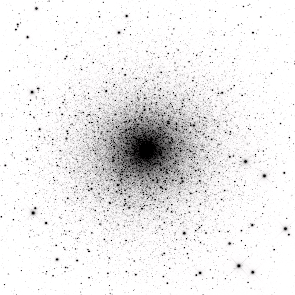
\includegraphics[width = 0.3\tw]{m13.pdf}
    \caption{Шаровое скопление M13 (негатив)}
\end{wrapfigure}
\term{Шаровое звёздное скопление}~--- скопление звёзд, состоящее из нескольких сотен тысяч светил, тесно связанных гравитацией между собой. Обладают сферически симметричной формой, наблюдается увеличение концентрации звёзд ближе к центру скопления. Диаметр шаровых скоплений составляет 20\,--\,60~пк, а массы варьируется от $10^4$\,--\,$10^6$~солнечных. 

В галактике Млечный путь насчитывается всего около 160 шаровых звёздных скоплений. В отличие от рассеянных звёздных скоплений, шаровые располагаются не в плоскости галактического диска, а в гало.

Шаровые звёздные скопления гораздо старше рассеянных. Диаграммы Герцшпрунга--Рассела демонстрируют, что яркие звёзды вплоть до звёзд, похожих на Солнце, уже сошли с главной последовательности, \lookPicRef{pic:hr-globular-clusters}, что даёт оценку на возраст таких скоплений порядка 10~миллиардов лет.

\begin{figure}[h!]
    \begin{subcaptionblock}{0.48\tw}
        \centering
        \tikzsetnextfilename{hr-47-Tuc}
        \begin{tikzpicture}
            \begin{axis}[
                height = 4.5cm,
                width  = 1.05\tw,
                xlabel = {$B-V$},
                ylabel = {$M_V$},
                ymax   = 6.0,
                ymin   = -2.0,
                y dir  = reverse,
                xmax   = 1.75,
                xmin   = 0.25
            ]
                \addplot+[only marks, mark = o, mark options={scale=0.2, black}] table[x=B-V, y=M_V, col sep = comma]{data/hr-47-Tuc.csv};
            \end{axis}
        \end{tikzpicture}
        \caption{47\,Tuc}
    \end{subcaptionblock}
    \hfill
    \begin{subcaptionblock}{0.48\tw}
        \centering
        \tikzsetnextfilename{hr-m13}
        \begin{tikzpicture}
            \begin{axis}[
                height = 4.5cm,
                width  = 1.05\tw,
                xlabel = {$B-V$},
                ylabel = {$M_V$},
                ymax   = 8.0,
                ymin   = -2.0,
                y dir  = reverse,
                xmax   = 1.25,
                xmin   = -0.25
            ]
                \addplot+[only marks, mark = o, mark options={scale=0.2, black}] table[x=B-V, y=M_V, col sep = comma]{data/hr-M13.csv};
            \end{axis}
        \end{tikzpicture}
        \caption{M13}
        \label{pic:hr-m13}
    \end{subcaptionblock}
    \caption{Диаграммы Герцшпрунга--Рассела шаровых звёздных скоплений}
    \label{pic:hr-globular-clusters}
\end{figure}

Помимо диаграммы Герцшпрунга--Рассела о внушительном возрасте говорит температура самых холодных белых карликов. Так возраст шарового звёздного скопления M4 оценивается в 12.7~миллиардов лет~\cite{whiteDwarfCooling}.
 
Внимательный читатель мог заметить, что, согласно \picRef{pic:hr-m13}, в шаровом звёздном скоплении M13 присутствует некоторое количество горячих ярких звёзд, возраст которых должен быть сильно меньше оценок возраста скоплений. Такие звёзды называются \term{голубыми отстающими}, они формируются в результате слияния звёзд или перетекания вещества между звёздами в центре скоплений, где звёзды располагаются наиболее плотно.
 
